\begin{tabular}{@{}l@{~~}l@{}}

  
\begin{tikzpicture}[scale=0.8]
    \def\printonlylargeenough#1#2{\unless\ifdim#2pt<#1pt\relax
      #2\printnumbertrue
      \else
      \printnumberfalse
      \fi}
    \newif\ifprintnumber
    \pie[rotate=120, radius=3, before number=\printonlylargeenough{10}, after number=\ifprintnumber\%\fi]{26.2/\normalsize get, 17.8/\normalsize put, 12.9/\normalsize remove, 43.2/\normalsize \textit{\shortstack[c]{others\\(98)}}}
    \node () at (-.2,-4) {\bf\normalsize\code{ConcurrentHashMap}};
  \end{tikzpicture}

  &

  
\begin{tikzpicture}[scale=0.8]
    \def\printonlylargeenough#1#2{\unless\ifdim#2pt<#1pt\relax
      #2\printnumbertrue
      \else
      \printnumberfalse
      \fi}
    \newif\ifprintnumber
    \pie[rotate=120, radius=3, before number=\printonlylargeenough{10}, after number=\ifprintnumber\%\fi]{30.7/\normalsize add, 21.0/\normalsize contains, 19.1/\normalsize remove, 29.2/\normalsize \textit{\shortstack[c]{others\\(17)}}}
    \node () at (-.2,-4) {\bf\normalsize\code{ConcurrentSkipListSet}};
  \end{tikzpicture}
\\

  
\begin{tikzpicture}[scale=0.8]
    \def\printonlylargeenough#1#2{\unless\ifdim#2pt<#1pt\relax
      #2\printnumbertrue
      \else
      \printnumberfalse
      \fi}
    \newif\ifprintnumber
    \pie[rotate=100, radius=3, before number=\printonlylargeenough{10}, after number=\ifprintnumber\%\fi]{28.6/\normalsize add, 24.4/\normalsize size, 11.7/\normalsize poll, 35.3/\normalsize \textit{\shortstack[c]{others\\(24)}}}
    \node () at (-.2,-4) {\bf\normalsize\code{ConcurrentLinkedQueue}};
  \end{tikzpicture}

  &

  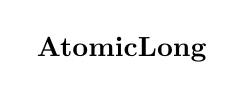
\begin{tikzpicture}[scale=0.8]
    \def\printonlylargeenough#1#2{\unless\ifdim#2pt<#1pt\relax
      #2\printnumbertrue
      \else
      \printnumberfalse
      \fi}
    \newif\ifprintnumber
    \pie[rotate=115, radius=3, before number=\printonlylargeenough{10}, after number=\ifprintnumber\%\fi]{37.3/\normalsize get, 15.6/\normalsize incrementAndGet, 14.3/\normalsize set, 32.8/\normalsize \textit{\shortstack[c]{others\\(137)}}}
    \node () at (-.2,-4) {\bf\normalsize\code{AtomicLong}};
  \end{tikzpicture}

\end{tabular}
